\documentclass[12pt,a4paper]{article}
\usepackage{amsmath,amssymb,graphicx,float}
\usepackage[margin=2cm]{geometry}
\usepackage{hyperref}
\usepackage[utf8]{inputenc}
\usepackage{enumitem}
\usepackage{multicol}
\usepackage{booktabs}

\title{\textbf{Physics 12 Formulas}\\\large Fundamental Constants and Equations}
\date{}

\begin{document}

\maketitle

\section{Physics Formulas}

\subsection{CH1,2,3: Kinematics}
\begin{align*}
  \begin{array}{l@{\hspace{2cm}}l@{\hspace{2cm}}l}
    \vec{v} = \vec{v}_0 + \vec{a}t & \bar{v} = \frac{\vec{v} + \vec{v}_0}{2} & v^2 = v_0^2 + 2\vec{a} \cdot \vec{d} \\[1em]
    \vec{d} = \vec{v}_0t + \frac{1}{2}\vec{a}t^2 & d = \left(\frac{v_f + v_i}{2}\right)t & v_x = v \cos \theta \\[1em]
    v_y = v \sin \theta & v = \sqrt{v_x^2 + v_y^2} & \theta = \tan^{-1}\left(v_y / v_x\right) \\[1em]
    h = \frac{v_{0y}^2}{2g} & R = \frac{v_0^2 \sin 2\theta_0}{g} & \text{(max when }\theta_0 = 45^\circ\text{)}
  \end{array}
\end{align*}

\subsection{CH4,5,9: Dynamics}
\begin{align*}
\begin{array}{l@{\hspace{1cm}}l@{\hspace{1cm}}l}
\vec{F}_\text{net} = m\vec{a} & \vec{F}_\text{net} = \vec{F}_\text{applied} - \vec{F}_\text{against} & \vec{F}_g = m\vec{g} 
\\[1em]
\vec{F}_\text{fr} = \mu \vec{F}_N & T=\frac{F_{\perp}}{2 \sin (\theta)} & \Delta L=\frac{1}{Y} \frac{F}{A} L_0 \\[1em]
w_{\|}=w \sin (\theta)=m g \sin (\theta) & w_{\perp}=w \cos (\theta)=m g \cos (\theta) & F_{\mathrm{D}}=\frac{1}{2} \mathrm{C} \rho A v^2 \\[1em]
\mathrm{MA}=\frac{F_{\mathrm{o}}}{F_{\mathrm{i}}}=\frac{l_{\mathrm{i}}}{l_{\mathrm{o}}} & \tau=r F \sin \theta & 
\end{array}
\end{align*}

\subsection{CH6: Circular Motion and Gravity}
\begin{align*}
\begin{array}{l@{\hspace{2cm}}l}
\Delta \theta=\frac{\Delta s}{r} & v=r \omega \text{ or } \omega=\frac{v}{r} \\[1em]
a_{\mathrm{c}}=\frac{v^2}{r} = r \omega^2 & F_{\mathrm{c}}=m a_{\mathrm{c}}=m \frac{v^2}{r}=m r \omega^2 \\[1em]
F=G \frac{m M}{r^2} & \frac{T_1^2}{T_2^2}=\frac{r_1^3}{r_2^3}, \: T^2=\frac{4 \pi^2}{G M} r^3
\end{array}
\end{align*}

\subsection{CH7: Work, Energy, and Power}

\begin{align*}
  \begin{array}{l@{\hspace{2cm}}l@{\hspace{2cm}}l}
    W = \vec{F} \cdot \vec{d} & E_p = mgh & E_k = \frac{1}{2}mv^2 \\[1em]
    P = \frac{W}{t} & \Delta E = E_f - E_i &
  \end{array}
\end{align*}

\subsection{CH8: Momentum}

\begin{align*}
  \begin{array}{l@{\hspace{2cm}}l@{\hspace{2cm}}l}
    \vec{p} = m\vec{v} & \Delta \vec{p} = \vec{F}\Delta t & m_T \vec{V}_T = m_1 \vec{v}_1 + m_2 \vec{v}_2 \\
    a=\frac{v_{\mathrm{e}}}{m} \frac{\Delta m}{\Delta t}-g & v=v_{\mathrm{e}} \ln \frac{m_0}{m_{\mathrm{r}}} &
  \end{array}
\end{align*}

\subsection{CH18: Electrostatics - Electric Forces and Fields}
\begin{align*}
\begin{array}{l@{\hspace{2cm}}l}
\vec{F}_E = k\frac{|q_1 q_2|}{r^2}\hat{r} & \vec{E} = \frac{\vec{F}}{q} = k\frac{|Q|}{r^2}\hat{r} \\[1em]
\end{array}
\end{align*}

\subsection{CH19: Electric Potential and Capacitance}
\begin{align*}
\begin{array}{l@{\hspace{1.5cm}}l}
E_p = \frac{kq_1 q_2}{r}, \quad \Delta PE = q\Delta V & V = \frac{kQ}{r}, \quad V_{AB} = Ed \text{ (uniform field)} \\[1em]
\vec{E} = -\frac{\Delta V}{\Delta s}\hat{r} & C = \frac{Q}{V}\quad = \varepsilon_0\frac{A}{d} \text{ (parallel)}\quad = \kappa\varepsilon_0\frac{A}{d} \text{ (dielectric)} \\[1em]
\frac{1}{C_s} = \frac{1}{C_1} + \frac{1}{C_2} + \cdots, \quad C_p = C_1 + C_2 + \cdots & E_{cap} = \frac{QV}{2} = \frac{CV^2}{2} = \frac{Q^2}{2C}
\end{array}
\end{align*}


\subsection{CH20: Current and Resistance}
\begin{align*}
\begin{array}{l@{\hspace{1.5cm}}l}
I = \frac{\Delta Q}{\Delta t}, = nqAv_d & \text{Ohm's Law: } I = \frac{V}{R}, \quad V = IR \\[1em]
R = \frac{\rho L}{A}, \quad \rho = \rho_0(1+\alpha \Delta T), \quad R = R_0(1+\alpha \Delta T) & P = IV = I^2R = \frac{V^2}{R}, \quad E = Pt \\[1em]
\text{AC: } V = V_0\sin 2\pi ft, \quad I = I_0\sin 2\pi ft & V_{\text{rms}} = \frac{V_0}{\sqrt{2}}, \quad I_{\text{rms}} = \frac{I_0}{\sqrt{2}}, \quad P_{\text{ave}} = I_{\text{rms}}V_{\text{rms}}
\end{array}
\end{align*}

\subsection{CH21: Circuits}
\begin{align*}
\begin{array}{l@{\hspace{1.5cm}}l}
\text{Series: } R_s = R_1 + R_2 + \cdots, \quad I_1 = I_2 = \cdots & \text{Parallel: } \frac{1}{R_p} = \frac{1}{R_1} + \frac{1}{R_2} + \cdots, \quad V_1 = V_2 = \cdots \\[1em]
\text{Terminal voltage: } V = \text{emf} - Ir & \text{Kirchhoff's Rules: } \sum I_{\text{in}} = \sum I_{\text{out}}, \quad \sum \Delta V = 0 \\[1em]
 V = \text{emf}(1-e^{-t/\tau}) \text{ (chrg)}, = V_0 e^{-t/\tau} \text{ (dischrg)} & \text{RC Circuits: } \tau = RC 
\end{array}
\end{align*}

\subsection{CH22: Magnetism}
\begin{align*}
  \begin{array}{l@{\hspace{1.5cm}}l}
    \vec{F} = Q\vec{v} \times \vec{B} = I\vec{L} \times \vec{B} & F = qvB\sin\theta \\[1em]
    \vec{B} = \frac{\mu_0 I}{2\pi r}\hat{\phi} & B_{\text{loop}} = \frac{\mu_0 I}{2r} \\[1em]
    B_{\text{solenoid}} = \mu_0 nI & r = \frac{mv}{qB} \\[1em]
    \tau = NIAB\sin\theta & \varepsilon_{\text{Hall}} = Blv \\[1em]
    \mu_0 = 4\pi \times 10^{-7} \text{ T}\cdot\text{m/A} & \\
  \end{array}
\end{align*}

\subsection{CH23: Electromagnetic Induction}
\begin{align*}
  \begin{array}{l@{\hspace{1.5cm}}l}
    \Phi = \vec{B} \cdot \vec{A} = BA\cos\theta & \mathcal{E} = -N\frac{d\Phi}{dt} \\[1em]
    \vec{\mathcal{E}} = \vec{v} \times \vec{B} & \text{emf} = Bl\nu \\[1em]
    \text{emf}_0 = NAB\omega & V_{\text{back}} = \mathcal{E} - Ir \\[1em]
    \frac{V_s}{V_p} = \frac{N_s}{N_p} = \frac{I_p}{I_s} & \\
  \end{array}
\end{align*}

\iffalse

\subsection{CH20,21: Electric Circuits}
\begin{align*}
  \begin{array}{l@{\hspace{2cm}}l@{\hspace{2cm}}l}
    I = \frac{Q}{\Delta t} & V = IR & V_\text{terminal} = \mathcal{E} \pm Ir \\[1em]
    P = VI & &
  \end{array}
\end{align*}



\subsection{CH28: Relativity}
\begin{align*}
  \begin{array}{l@{\hspace{2cm}}l@{\hspace{2cm}}l}
    t = \frac{t_0}{\sqrt{1-\frac{v^2}{c^2}}} & L = L_0\sqrt{1-\frac{v^2}{c^2}} & m = \frac{m_0}{\sqrt{1-\frac{v^2}{c^2}}} \\[1em]
    u = \frac{v+u'}{1+\frac{vu'}{c^2}} & E = mc^2 & E_k = \frac{1}{2}mv^2
  \end{array}
\end{align*}


\fi


\newpage
\section{Mathematical Formulas}

\subsection{Right-angled Triangles}

\begin{figure}[H]
    \centering
    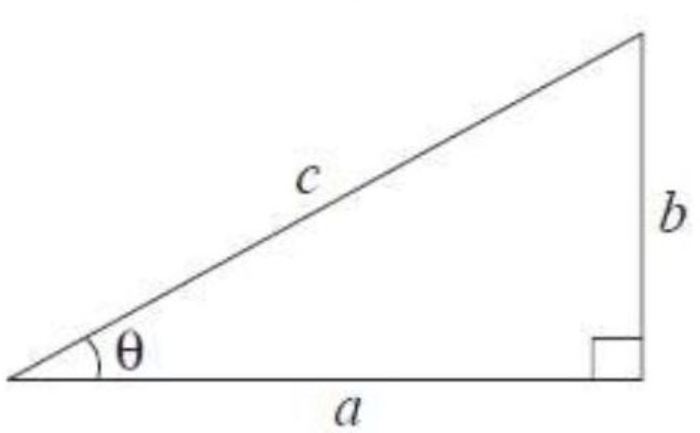
\includegraphics[width=0.4\linewidth]{12 Formula/rt.png}
    \caption{Right-angled triangle}
    \label{fig:Right-angled triangle}
\end{figure}

\begin{align*}
  \begin{array}{l@{\hspace{2cm}}l@{\hspace{2cm}}l}
    a^2 + b^2 = c^2 & \sin \theta = \frac{b}{c} & \cos \theta = \frac{a}{c} \\[1em]
    \tan \theta = \frac{b}{a} & \text{area} = \frac{1}{2}ab &
  \end{array}
\end{align*}

\subsection{All Triangles}
\begin{figure}[H]
    \centering
    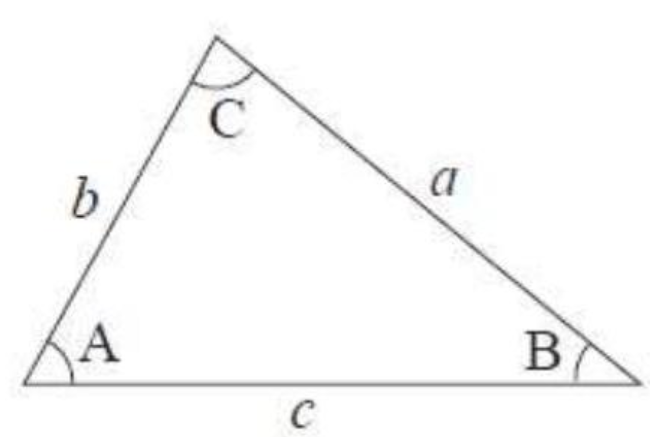
\includegraphics[width=0.4\linewidth]{12 Formula/nrt.png}
    \caption{Non-Right-angled triangle}
    \label{fig:Non-Right-angled triangle}
\end{figure}

\begin{align*}
  \begin{array}{l@{\hspace{2cm}}l@{\hspace{2cm}}l}
    \text{area} = \frac{1}{2} \text{base} \times \text{height} & \text{Sine Law:} \quad \frac{\sin A}{a} = \frac{\sin B}{b} = \frac{\sin C}{c} & \\[1em]
    \text{Cosine Law:} \quad c^2 = a^2 + b^2 - 2ab \cos C & &
  \end{array}
\end{align*}

\subsection{Circle and Sphere}
\begin{align*}
  \begin{array}{l@{\hspace{2cm}}l@{\hspace{2cm}}l}
    \text{Circle circumference:} \quad 2\pi r & \text{Circle area:} \quad \pi r^2 & \text{Sphere surface area:} \quad 4\pi r^2 \\[1em]
    \text{Sphere volume:} \quad \frac{4}{3}\pi r^3 & &
  \end{array}
\end{align*}

\subsection{Quadratic Equation}
For $ax^2 + bx + c = 0$: 
\[x = \frac{-b \pm \sqrt{b^2 - 4ac}}{2a}\]

\section{Metric Prefixes and Cardinal Directions}
\begin{figure}[H]
    \centering
    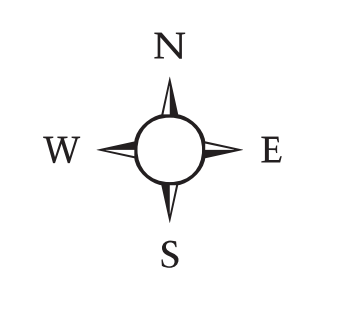
\includegraphics[width=0.4\linewidth]{12 Formula/nesw.png}
    \caption{Cardinal directions: North, South, East, and West}
    \label{fig:Cardinal directions}
\end{figure}

\begin{table}[H]
\centering
\begin{tabular}{@{}llcc@{}}
\toprule
Prefix & Symbol & Numerical & Exponential \\
\midrule
mega & M & 1000000 & $10^6$ \\
kilo & k & 1000 & $10^3$ \\
hecto & h & 100 & $10^2$ \\
deca & da & 10 & $10^1$ \\
 &  & 1 & $10^0$ \\
deci & d & 0.1 & $10^{-1}$ \\
centi & c & 0.01 & $10^{-2}$ \\
milli & m & 0.001 & $10^{-3}$ \\
micro & $\mu$ & 0.000001 & $10^{-6}$ \\
\bottomrule
\end{tabular}
\end{table}

\section{Fundamental Constants and Physical Data}

\begin{align*}
  \begin{array}{l@{\hspace{1cm}}r}
    \text{Gravitational constant:} & G=6.67 \times 10^{-11} \mathrm{Nm}^2/\mathrm{kg}^2 \\[1em]
    \text{Coulomb's Law constant:} & k=8.99 \times 10^9 \mathrm{Nm}^2/\mathrm{C}^2 \\[1em]
    \text{Elementary charge:} & e=1.60 \times 10^{-19} \mathrm{C} \\[1em]
    \text{Electron mass:} & m_e=9.11 \times 10^{-31} \mathrm{kg} \\[1em]
    \text{Proton mass:} & m_p=1.67 \times 10^{-27} \mathrm{kg} \\[1em]
    \text{Avogadro's Number:} & N_A=6.022 \times 10^{23} \mathrm{kg} \\[1em]
    \text{Permeability of free space:} & \mu_0=4\pi \times 10^{-7} \mathrm{Tm}/\mathrm{A} \\[1em]
    \text{Permittivity of free space:} & \varepsilon_0 = 8.85 \times 10^{-12} \mathrm{F}/\mathrm{m} \\[1em]
    \text{Speed of light:} & c=3.00 \times 10^8 \mathrm{m}/\mathrm{s} \\[1em]
    \text{Density of air:} & \rho=1.21 \mathrm{~kg} / \mathrm{m}^3 \\[1em]
    \text{Boltzmann constant:} & k_B=1.38 \times 10^{-23} \mathrm{J}/\mathrm{K}
  \end{array}
\end{align*}

\subsection{Earth}
\begin{align*}
  \begin{array}{l@{\hspace{1cm}}r@{\hspace{1cm}}l@{\hspace{1cm}}r}
    \text{Radius:} & 6.38 \times 10^6 \mathrm{m} & \text{Mass:} & 5.98 \times 10^{24} \mathrm{kg} \\[1em]
    \text{Surface gravity:} & g=9.81 \mathrm{m}/\mathrm{s}^2 & \text{Rotation period:} & 8.61 \times 10^4 \mathrm{s} \\[1em]
    \text{Orbit radius (Sun):} & 1.50 \times 10^{11} \mathrm{m} & \text{Orbit period (Sun):} & 3.16 \times 10^7 \mathrm{s}
  \end{array}
\end{align*}

\subsection{Moon}
\begin{align*}
  \begin{array}{l@{\hspace{1cm}}r@{\hspace{1cm}}l@{\hspace{1cm}}r}
    \text{Radius:} & 1.74 \times 10^6 \mathrm{m} & \text{Mass:} & 7.35 \times 10^{22} \mathrm{kg} \\[1em]
    \text{Rotation period:} & 2.36 \times 10^6 \mathrm{s} & \text{Orbit radius (Earth):} & 3.84 \times 10^8 \mathrm{m} \\[1em]
    \text{Orbit period (Earth):} & 2.36 \times 10^6 \mathrm{s} & &
  \end{array}
\end{align*}

\subsection{Sun}
Mass: $1.98 \times 10^{30} \mathrm{kg}$

\end{document}